\documentclass{article}
\usepackage{makeidx}
\usepackage{graphicx}
\usepackage{titlesec}
\setcounter{secnumdepth}{4}
\usepackage[utf8]{inputenc}

\title{mycc - My own C++ compiler implementation}
\author{Hanze Chen}
\date{January 2022}
\makeindex

\begin{document}
\maketitle
\section{Introduction}
    \begin{figure}[hb!]
        \centering
        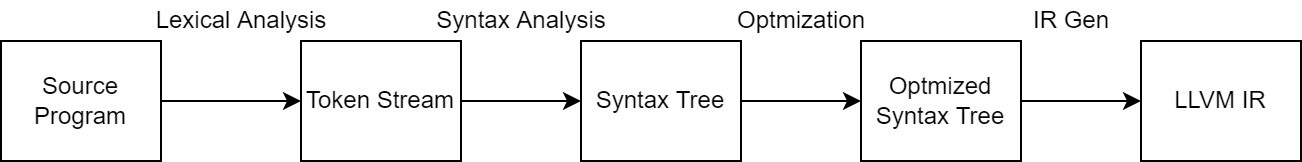
\includegraphics[width=10cm]{figure/frontend_structure.png}
        \caption{Frontend Structure}
        \label{Fig:frontend_structure}
    \end{figure}
\section{Implemented Function}
\subsection{Part0}

\section{Main Data Structures}
    \subsection{Lexical}
        \subsubsection{LexicalToken \index{Lexical Token Class}}
            Currently the following tokens are supported to recognized: \par
            \begin{table}[hb!]
                \centering
                \begin{tabular}{l|lll}
                    \hline
                    Token Type  & Regex                                                  & Example           & Description    \\ \hline
                    add         & \textbackslash{}\textbackslash{}+                      & +                 & Addition       \\
                    sub         & -                                                      & -                 & Subtraction    \\
                    mul         & \textbackslash{}\textbackslash{}*                      & *                 & Multiplication \\
                    div         & /                                                      & /                 & Division       \\
                    number      & {[}0-9{]}+\textbackslash{}\textbackslash{}.?{[}0-9{]}* & 0, 0.1 etc.       & Numbers        \\
                    Identifiers & {[}a-zA-Z\_{]}{[}a-zA-Z0-9\_{]}*                       & "a", "while" etc. & Identifiers    \\ \hline
                \end{tabular}
                \caption{Supported Token Type}
                \label{table:supported_lexical_token_list}
            \end{table}
    \subsection{Utils}
        \subsubsection{Status \index{Status Class}}
\printindex
\end{document}